\documentclass[a4paper,12pt]{article}

% --- 版式必须只加载一次，并放靠前 ---
\usepackage[a4paper,margin=2.5cm]{geometry}

% --- 中文与字体（ctex 内含 fontspec/xeCJK，适合 XeLaTeX）---
\usepackage{ctex}

% --- 数学与图形 ---
\usepackage{amsmath}
\usepackage{amssymb}      % 提供 \mathbb 等
\usepackage{graphicx}     % 插图（支持 pdf/png/jpg）
\usepackage{caption}
\usepackage{subcaption}
\usepackage{svg}
\usepackage{float} 

\graphicspath{{images_in_paper/}}
\DeclareGraphicsExtensions{.pdf,.png,.jpg}


% --- 表格 ---
\usepackage{booktabs}
\usepackage{array}
\usepackage{threeparttable}
\usepackage{subcaption}
% --- 目录样式（不要再加载 geometry）---
\usepackage{tocloft}

% --- 标题样式 ---
\usepackage{titlesec}

% --- 收紧itemize块 ---
\usepackage{enumitem}
\setlist{nosep}

% --- 页眉页脚（放在 geometry 之后）---
\usepackage{fancyhdr}
\setlength{\headheight}{15pt}
\pagestyle{fancy}
\fancyhf{}
\fancyfoot[C]{\thepage}

\newcommand{\teamID}{队伍控制号：NKUMMF2025138}
\fancyhead[R]{\teamID}

% section 中文编号 “一、”
\renewcommand\thesection{\chinese{section}}
\titleformat{\section}[block]
  {\centering\Large\bfseries}
  {\thesection\,、}
  {1em}{}

% subsection 继续用阿拉伯编号
\renewcommand\thesubsection{\arabic{section}.\arabic{subsection}}

% ======================================

\title{从时域到频域：基于多分支CNN网络的AI音频检测模型}
\author{NKUMMF2025138}
\date{}

\begin{document}
\maketitle
\thispagestyle{plain}  % 禁用摘要页的页眉，只保留页脚的页码

% \begin{center}
%     \textbf{\huge 摘\quad 要}
% \end{center}
% \vspace{1cm}  

\begin{abstract}
随着深度学习与生成模型的发展，AI 音乐创作在产业与艺术领域快速普及，但其版权归属、作品质量及可识别性等问题亟待解决。

本文提出一种基于多分支卷积神经网络（Multi-Branch CNN）的端到端 AI 音频检测与评分模型，从时域、频域及声学统计等多角度提取 11 类特征，分别经五个并行分支建模后融合判别。针对单分支贡献难以量化的问题，引入分支探针机制，基于各分支独立判别准确率确定加权系数，构建可解释的 AI 痕迹综合评分体系。

设计多种扰动与对抗性处理（如频谱均衡、高频注入、环境噪声混入等）评估模型鲁棒性，并结合分支贡献分析揭示其在时域包络与共振峰布局上的依赖性。实验结果表明，该模型在验证集上准确率可达 89\%–90\%，在多数轻中度扰动下保持稳定性能，综合评分在强扰动下亦具较高稳健性。本文方法具有较低计算开销与良好可扩展性，可推广至语音伪造检测、环境音识别等领域。
\end{abstract}
\vspace{1em}
\noindent\textbf{关键词：} AI 音乐检测；多分支CNN；音频特征提取；探针机制；AI 痕迹评分

\newpage  

\tableofcontents 
\newpage  

\section{模型建立与求解}
\subsection{问题1模型建立与求解}
本文从音频信息的时域、频域、全局统计量等角度，从原始音频文件中提取了十一个特征，
按类别分组后输入给多分支CNN网络，构建了融合多域信息的CNN分类器，
用于判别音频是否为AI生成的音乐作品。模型的判别准确率可以达到$89.24\% \pm 0.43\%$


\subsubsection{特征说明}
在特征提取阶段，本文将所有输入音频统一重采样为 22050 Hz，该频率在保留音频主要能量的同时有效降低了计算开销。为确保模型训练的稳定性，原始音频被切分为 20 秒的固定片段。

在数据处理流程中，系统会先将多格式音频转换为 WAV 格式以实现兼容，随后通过短时傅里叶变换（STFT）与梅尔滤波器组进行频谱分析，以模拟人耳的感知特性。最终，本文提取了涵盖时域、频域及声学结构的多种关键特征（见表 \ref{tab:audio-features}），以全面表征音频的能量、频谱形状及谐波等信息。

\begin{table}[h]
  \centering
  \begin{tabular}{lll lll}
    \toprule
    特征名称 & 维度 & 特征类型 & 特征名称 & 维度 & 特征类型 \\
    \midrule
    rms       & (1, 862)   & 时域能量    & zcr       & (1, 862)   & 时域变化       \\
    hjorth    & (3, 1)     & 全局统计    & log\_mel  & (128, 862) & 频域谱图       \\
    mfcc      & (13, 862)  & 声学特征    & centroid  & (1, 862)   & 频谱形状       \\
    contrast  & (7, 862)   & 频谱对比度  & flatness  & (1, 862)   & 频谱形状       \\
    f0        & (1440,)    & 音高曲线    & hnr       & (1998,)    & 声学质量       \\
    formant   & (3, 2000)  & 共振峰      & —         & —          & —             \\
    \bottomrule
  \end{tabular}
  \caption{各特征的名称、维度及类型}
  \label{tab:audio-features}
\end{table}

\subsubsection{模型建立}

本研究构建了一个多分支卷积神经网络（Multi-Branch CNN），用于融合处理多种类型的音频特征，从而实现对 AI 生成音频的准确识别。整体网络结构如下图所示，模型共由五个输入分支构成，分别对应不同特征类型，并通过特征融合实现最终的二分类判别。

\begin{figure}[h]
    \centering
    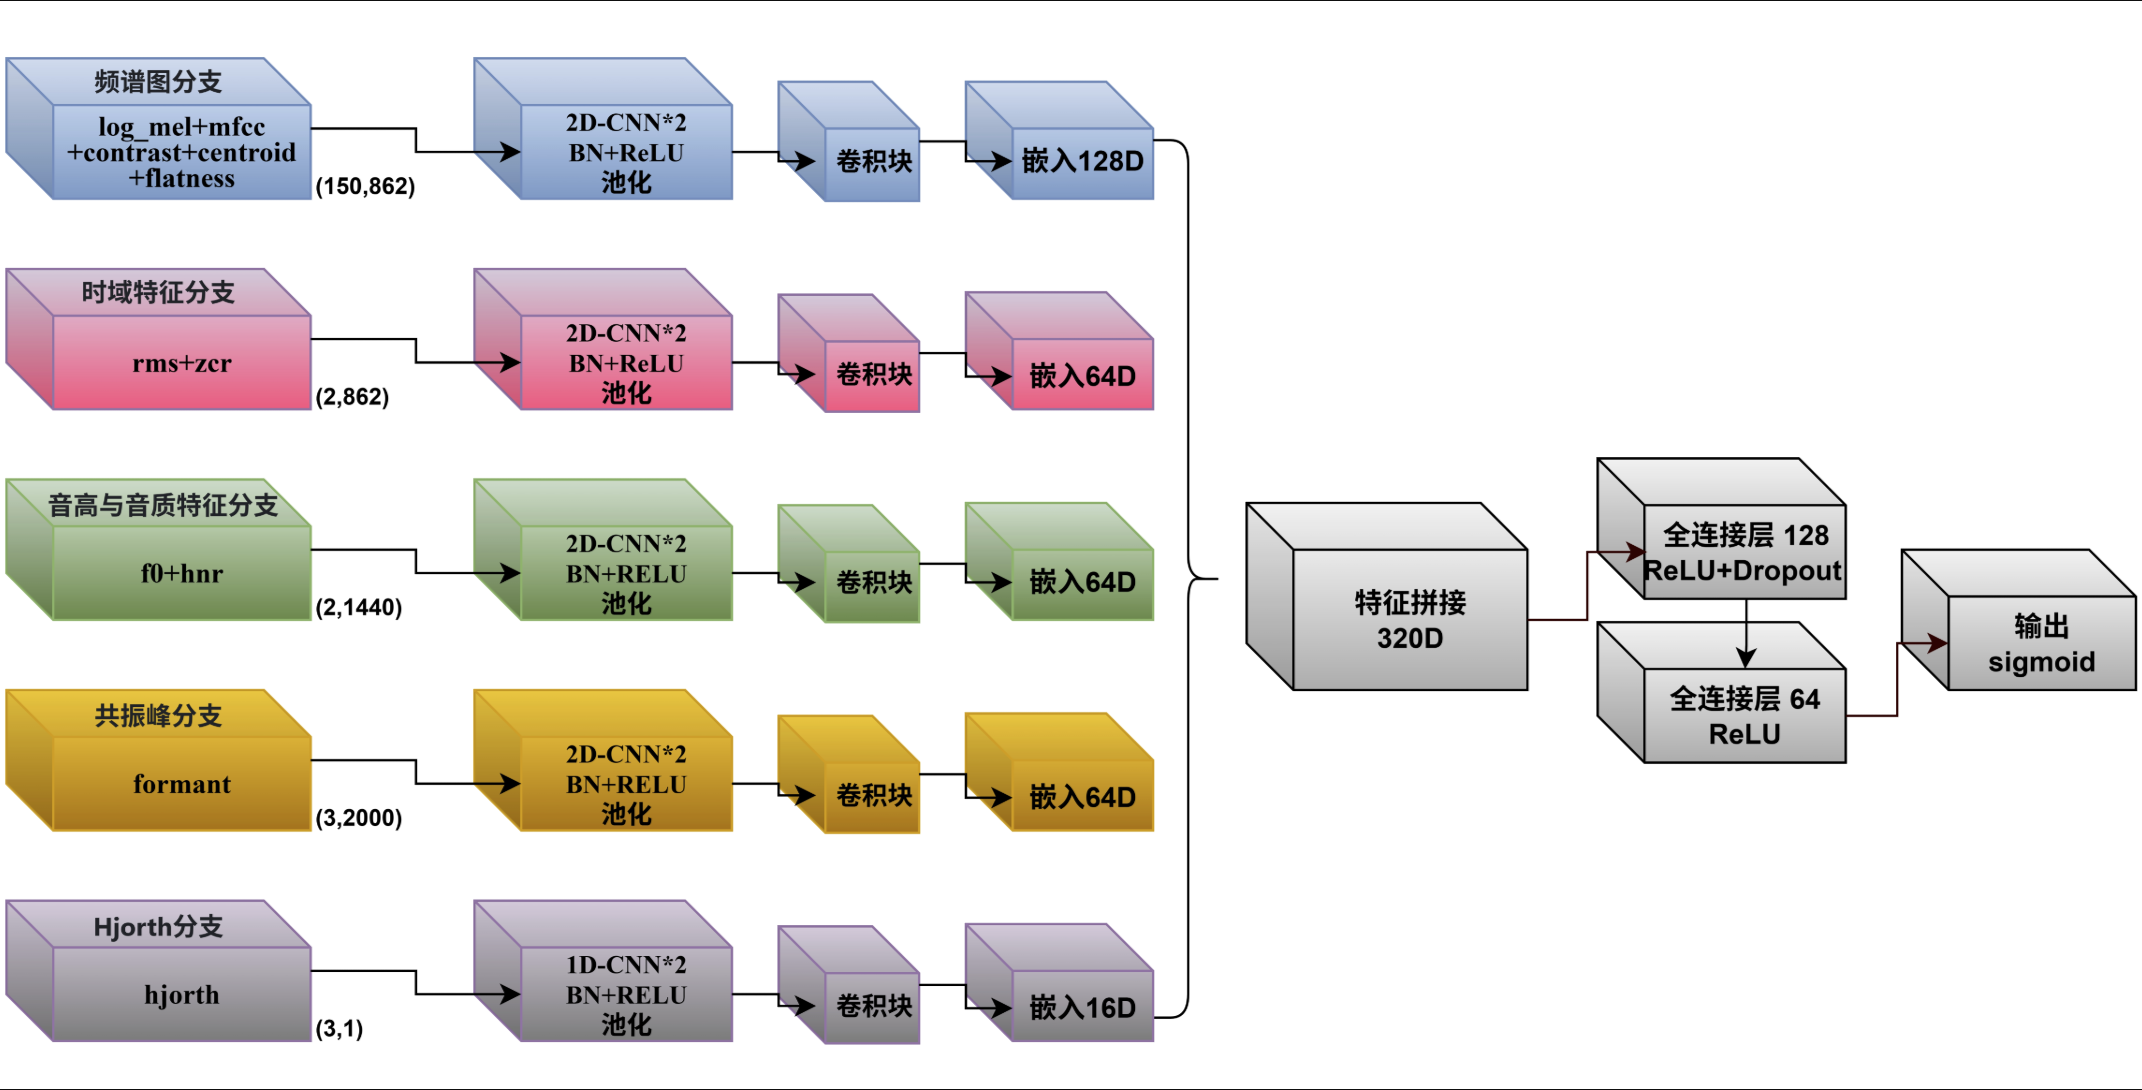
\includegraphics[width=0.75\linewidth]{images_in_paper/model.png}
    \caption{多分支CNN示意图}
    \label{fig:model}
\end{figure}

\begin{itemize}
 
  \item \textbf{频谱图分支（Spectrogram Branch）：} 输入由 \texttt{log\_mel} 频谱图（Log-Mel Spectrogram）、\texttt{mfcc}（Mel Frequency Cepstral Coefficients）、\texttt{contrast}（Spectral Contrast）、\texttt{centroid}（Spectral Centroid）以及 \texttt{Spectral Flatness}五种频域特征沿通道维度拼接形成的多通道频谱图。该分支通过两层二维卷积神经网络（2D CNN）提取其在时间与频率双维度上的局部模式，随后经全局平均池化获得固定长度的 64 维特征向量，并通过全连接层映射为 128 维表示。

    \item \textbf{时域分支：} 主要处理 \texttt{rms}（Root Mean Square Energy，均方根能量）和 \texttt{zcr}（Zero Crossing Rate，过零率）两类时域特征。输入形状为 $(2, 862)$，采用一维卷积（1D CNN）提取其时间结构，最终得到 64 维特征向量。
      
    \item \textbf{音高与音质分支：} 接收 \texttt{f0}（Fundamental Frequency，基频）与 \texttt{hnr}（Harmonics-to-Noise Ratio，谐噪比）两种声学特征，拼接后输入为 $(2, 1440)$，通过 1D CNN 提取其调型与音质模式，映射为 64 维向量。
      
    \item \textbf{共振峰分支：} 输入为 20s音频片段在各个时间窗口上的\texttt{formant}特征构成的三维序列，通过 1D CNN 处理后压缩为 64 维特征。
      
    \item \textbf{Hjorth 参数分支（Hjorth Parameter Branch）：} \texttt{hjorth} 特征为 $(3,1)$ 的全局统计量，包括 Activity（活动度，衡量信号能量）、Mobility（移动性，反映波形变化速度）与 Complexity（复杂度，描述波形不规则性），不含时间维度，因此直接使用两层全连接网络映射为 16 维表示。

\end{itemize}

五个分支提取的特征向量分别为：128维（频谱图）、64维（时域）、64维（音高音质）、64维（formant）与16维（hjorth），合并后得到一个 $336$ 维的全局音频表征。该向量随后输入至全连接分类器，包含一层隐藏层（64单元），使用 ReLU 激活与 Dropout 防止过拟合，最终输出一个概率值，判定音频是否为 AI 生成。



\subsubsection{结果与分析}
\noindent\textbf{数据可视化}\par
模型在200个epoch内的学习曲线如图~\ref{fig:acc-loss} 所示。随着训练代数的增加，训练准确率从76.5\%持续上升并最终收敛于88.5\%左右，训练损失呈单调递减趋势，最终趋近于0.27；验证准确率和损失虽经历多次波动，但最终趋于稳定，分别在89\%-90\%和0.25-0.26之间。单一指标对比下，经过多次训练的模型在验证集上的指标要优于训练集。

上述结果表明模型训练稳定，未出现过拟合迹象（如验证损失反弹、验证精度持续下降）。这说明多分支特征融合结构在提取不同维度音频信息时具有较好的泛化能力，能够有效捕捉AI生成音乐与人类创作音乐的差异特征。



\begin{figure}[htb]
  \centering
  \begin{subfigure}{0.48\linewidth}
    \centering
    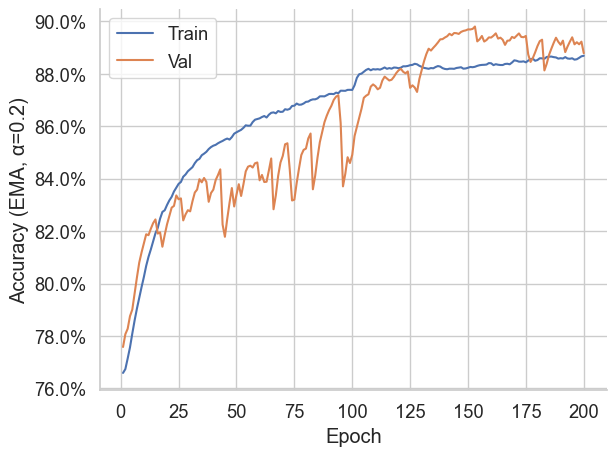
\includegraphics[width=\linewidth]{images_in_paper/acc_train_val.png}
    \caption{准确率（Train vs Val）}
    \label{fig:acc}
  \end{subfigure}\hfill
  \begin{subfigure}{0.48\linewidth}
    \centering
    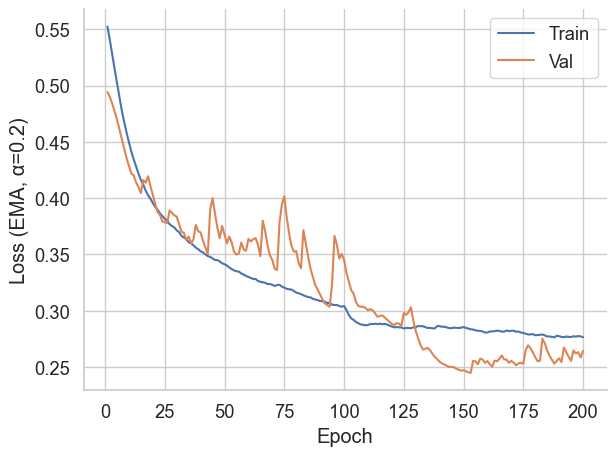
\includegraphics[width=\linewidth]{images_in_paper/loss_train_val.png}
    \caption{损失（Train vs Val）}
    \label{fig:loss}
  \end{subfigure}
  \caption{训练过程的准确率与损失对比}
  \label{fig:acc-loss}
\end{figure}


\subsection{问题3模型建立与求解}

本问旨在通过人为扰动与对抗性处理，评估模型在复杂场景下的鲁棒性，并探索提升检测性能的可解释性改进策略。实验流程包括扰动构造、稳健性评估及模型优化。

\subsubsection{扰动构造}
为系统性评估模型对微小音频变动的敏感度，本文设计了三类对抗性扰动策略：

\begin{enumerate}
    \item \textbf{多分支特征扰动}：针对音频的多维特征进行针对性微扰。包括：通过动态压缩与全通滤波引入时域非线性相位偏差；施加窄带均衡（EQ）产生频域偏移；模拟共振峰漂移及人声基频平移；引入白噪声以降低谐噪比（HNR）；以及通过微量时域伸缩改变节奏分布。
    \item \textbf{参数均衡器扰动}：基于二阶 IIR 滤波器组，通过预设的中心频率、增益（$\pm 2\,\text{dB}$）及品质因数进行参数化扰动。此类扰动确保主观听感的一致性，同时在特征空间内诱导分布偏移。
    \item \textbf{背景环境模拟}：将原始音频与环境背景声（如自然音效、环境白噪声）以不同信噪比进行线性叠加，以验证模型在真实复杂声学场景下的抗干扰能力。
\end{enumerate}

上述扰动均设置了多档强度，旨在平衡对抗样本的隐蔽性与模型判别的挑战性。


\subsubsection{鲁棒性分析}
为量化模型在复杂环境下的稳健性，本文构建了包含特征扰动、均衡器调节及背景噪声注入的三类对抗测试集。
实验设置 \texttt{mild} 至 \texttt{strong} 三档强度，
通过对比扰动前后模型输出概率（\texttt{prob\_main}）的相对降幅与方差变化，评估模型性能的抗干扰能力。重点分析高频注入、环境噪声及共振峰漂移等高风险场景，旨在揭示不同扰动类型对模型预测置信度的影响机制。

\begin{table}[H]
\centering
\caption{不同扰动类型下主分类概率与综合评分均值对比}
\label{tab:family-stats}
\begin{tabular}{lccc}
\toprule
扰动家族（Family） & 示例 & 样本数 & $\texttt{prob\_main}$均值 \\
\midrule
\textbf{comboAll}       & 多种扰动叠加版本                 & 1  & \textbf{0.764}\\
\textbf{pitchHNR}       & 微转调 + 谐噪比调整              & 1  & 0.659\\ 
\textbf{specEQ}         & 频谱均衡/倾斜（EQ）              & 7  & 0.604\\ 
\textbf{highFreqInject} & 高频注入（HI）                   & 8  & 0.461\\ 
\textbf{ambientNoise}   & 环境噪声混入（雨声、森林、城市） & 4  & 0.422\\ 
\textbf{other}          & 其他扰动方式                     & 13 & 0.411\\ 
\bottomrule
\end{tabular}
\end{table}

表 \ref{tab:family-stats} 显示不同扰动对模型判别准确性的影响存在显著差异。
其中 \texttt{comboAll} 与 \texttt{pitchHNR} 类扰动下模型表现相对稳定，
主分类概率分别维持在 0.764 与 0.659，体现了较强的稳健性。
相比之下，\texttt{specEQ} 造成性能轻微下滑；而 \texttt{highFreqInject} 与 
\texttt{ambientNoise} 对模型干扰尤为剧烈，分别将分类概率降至 0.461 与 0.422。
上述结果表明，高频注入与背景环境噪声是模型特征空间的薄弱环节，
是后续模型优化与增强鲁棒性的核心关注方向。





\subsubsection{归因分析：分支表征与扰动敏感性的关联}
为识别检测器对不同声学特征的依赖，我们在分支嵌入空间（即各CNN分支输入到全连接层的一维张量）进行了降维可视化，分析数据点在各个分支上的区域可分性，同时使用AUC、ACC、Fisher比率和logit等指标来量化分析各个分支对最终决策的贡献程度。

\paragraph{（1）区域可分性：时域分支更“可分”，formant 分支更“缠绕”。}
在图~\ref{fig:time_tsne} 中，时域嵌入出现了与主簇明显分离的红色带状簇，显示 AI 音频在\emph{能量包络/瞬态结构}维度存在系统性轨迹；
PCA（图~\ref{fig:time_pca}）虽线性可分性有限，但仍呈现出沿第一主轴的标签渐变。

\begin{figure}[H]
  \centering
  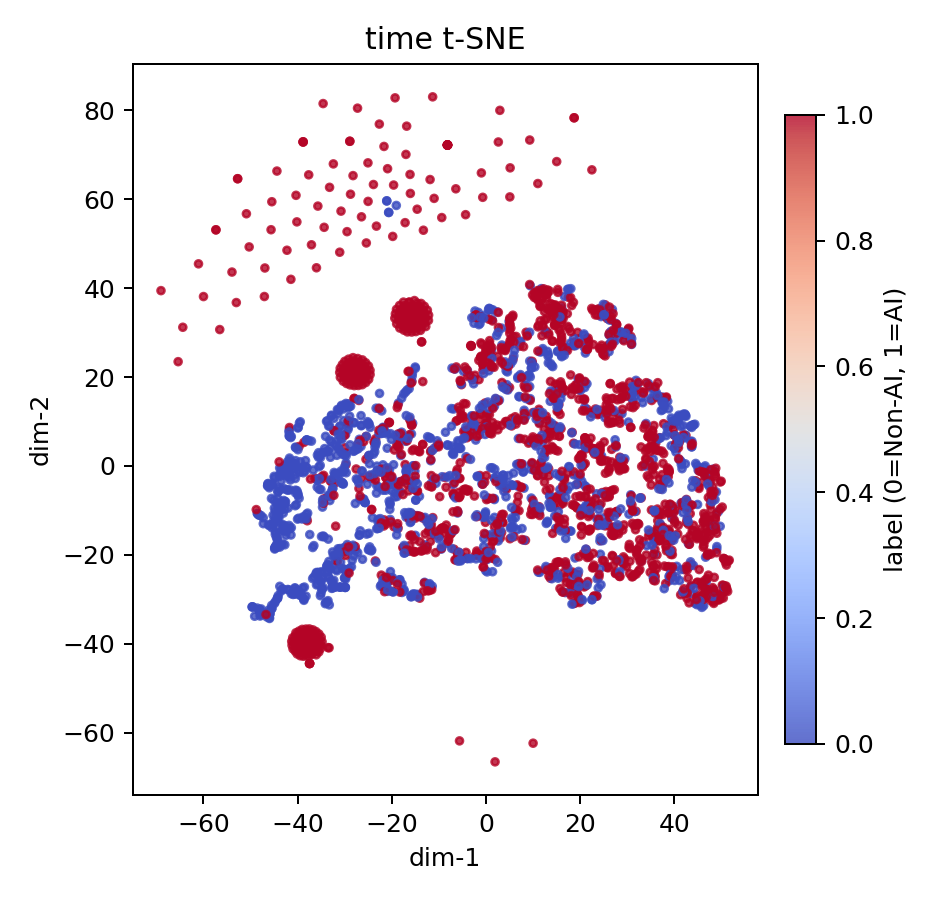
\includegraphics[width=.4\linewidth]{images_in_paper/embed_time_tsne.png}
  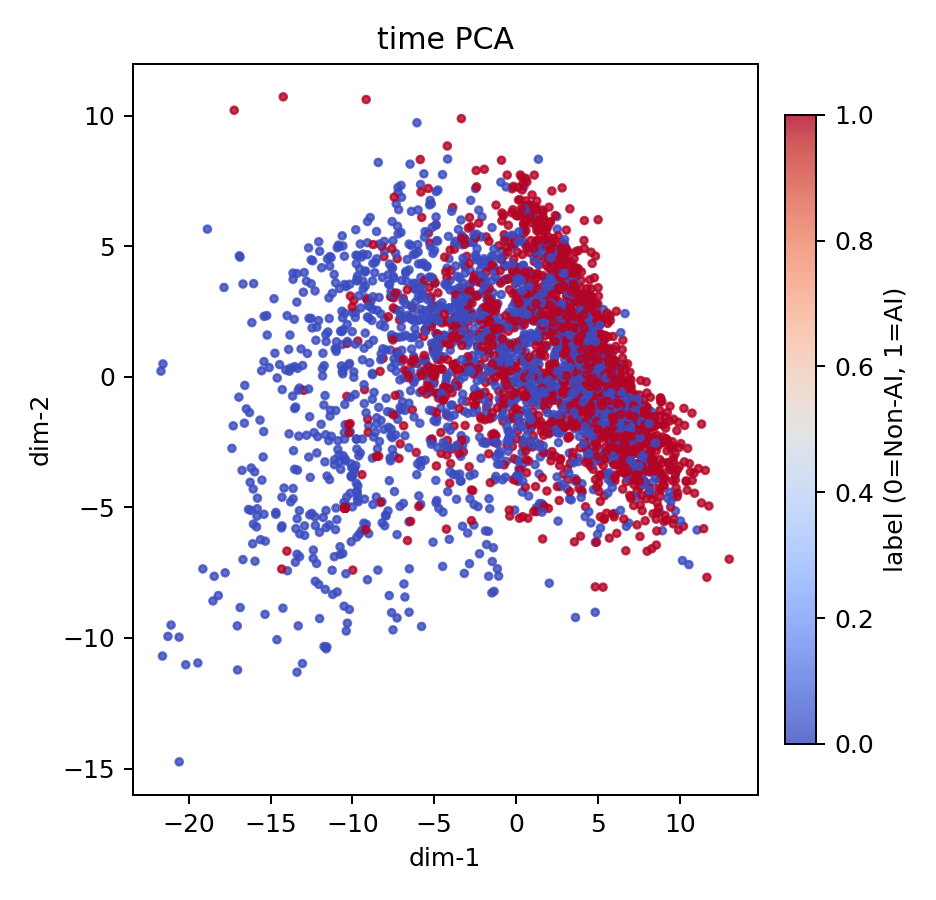
\includegraphics[width=.4\linewidth]{images_in_paper/embed_time_pca.png}
  \caption{时域分支嵌入：t-SNE（左）与 PCA（右）。}
  \label{fig:time_tsne}
  \label{fig:time_pca}
\end{figure}

相对地，formant 分支（图~\ref{fig:formant_tsne}）总体上红蓝高度交织，仅在若干局部“岛状”区域聚集，
表明\emph{整体}频谱包络并不足以稳定区分全部 AI 样式，但对特定风格（如固定声道/共振峰模板）的 AI 样本存在\emph{局部}可分性。

\begin{figure}[H]
  \centering
  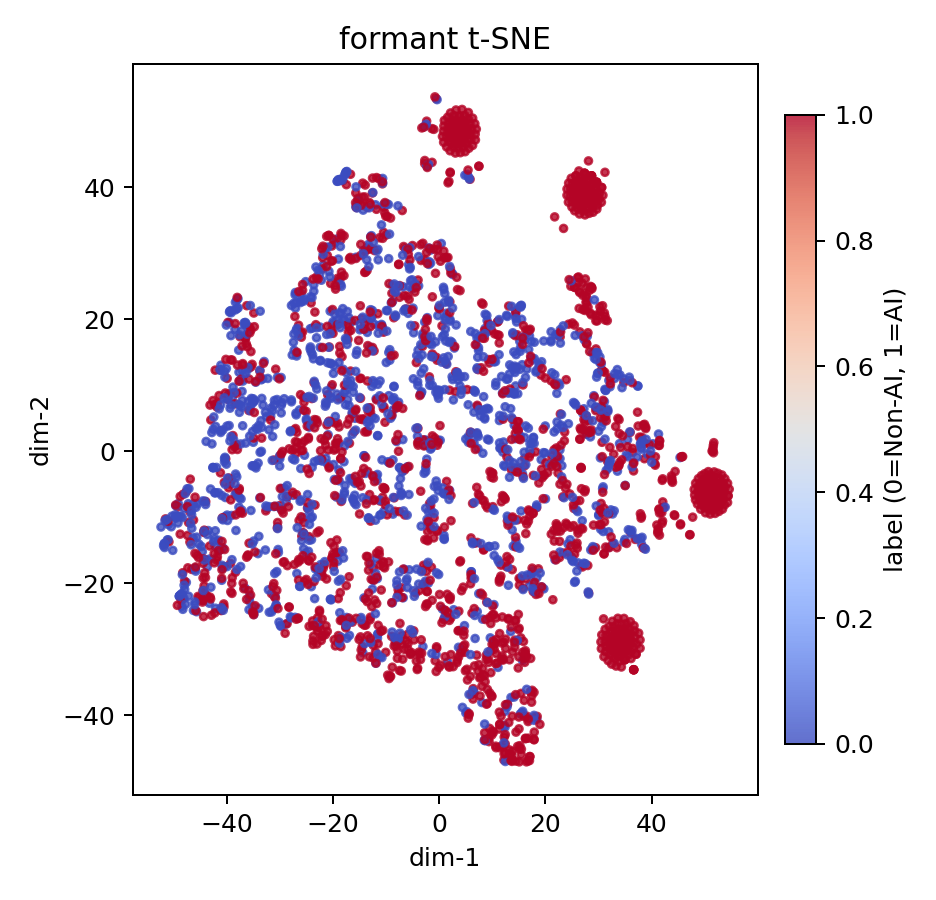
\includegraphics[width=.4\linewidth]{images_in_paper/embed_formant_tsne.png}
  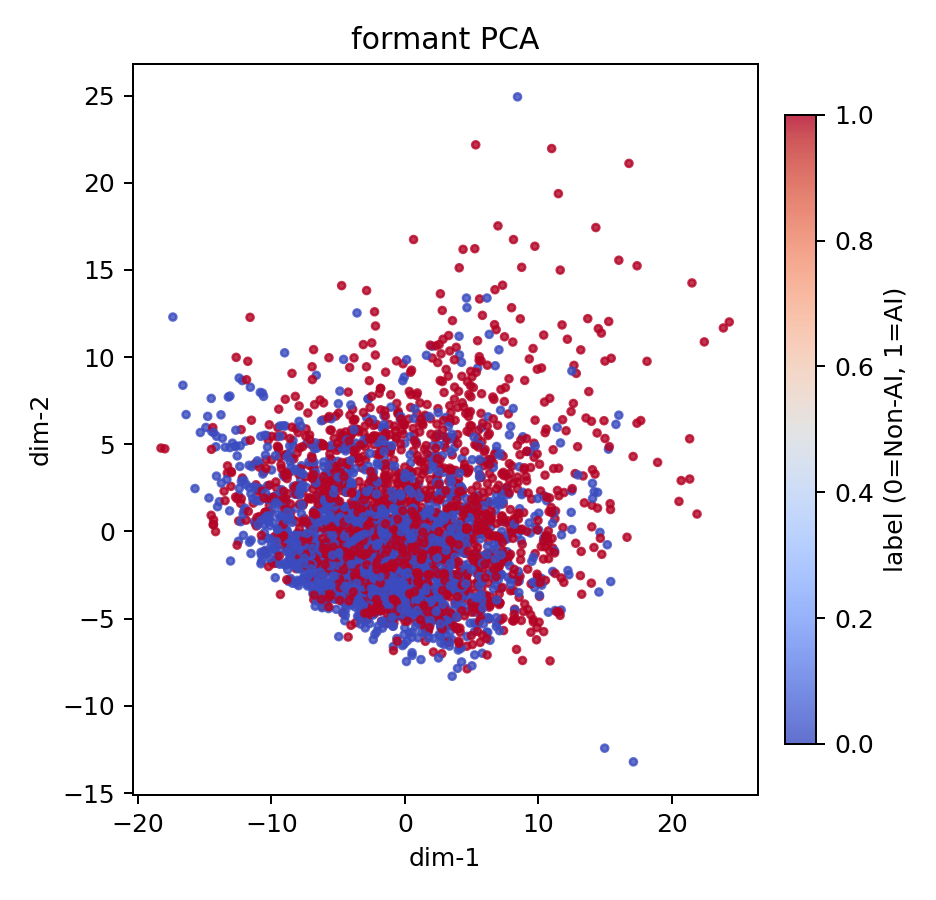
\includegraphics[width=.4\linewidth]{images_in_paper/embed_formant_pca.png}
  \caption{formant 分支嵌入：t-SNE（左）与 PCA（右）。}
  \label{fig:formant_tsne}
  \label{fig:formant_pca}
\end{figure}

\paragraph{（2）量化分析与贡献度归因}
扰动实验表明，针对特定分支的微扰能显著改变模型判别。\emph{时域动态}与\emph{类共振峰}扰动对 $\mathrm{prob\_main}$ 的压低作用最为显著，而高频窄带 EQ 影响较弱。这证实模型决策高度依赖时域包络与人声共振峰布局。

为进一步探究决策机理，本文通过线性层权重拆分（Contribution Analysis）分析各分支对最终判别力度（Logit）的贡献。图~\ref{fig:contrib_means} 的归因结果显示：\texttt{spec} 分支在 AI 样本中呈现显著正向贡献，是识别 AI 特征的核心；而 \texttt{time} 分支则起主要抑制作用。相比之下，\texttt{prosody}、\texttt{formant} 与 \texttt{hjorth} 的贡献幅值较小。实验证明，一旦对贡献度较高的关键特征执行结构性微调，模型决策边界将发生显著偏移，由 AI 区域转向“非 AI”区域。

\begin{figure}[H]
  \centering
  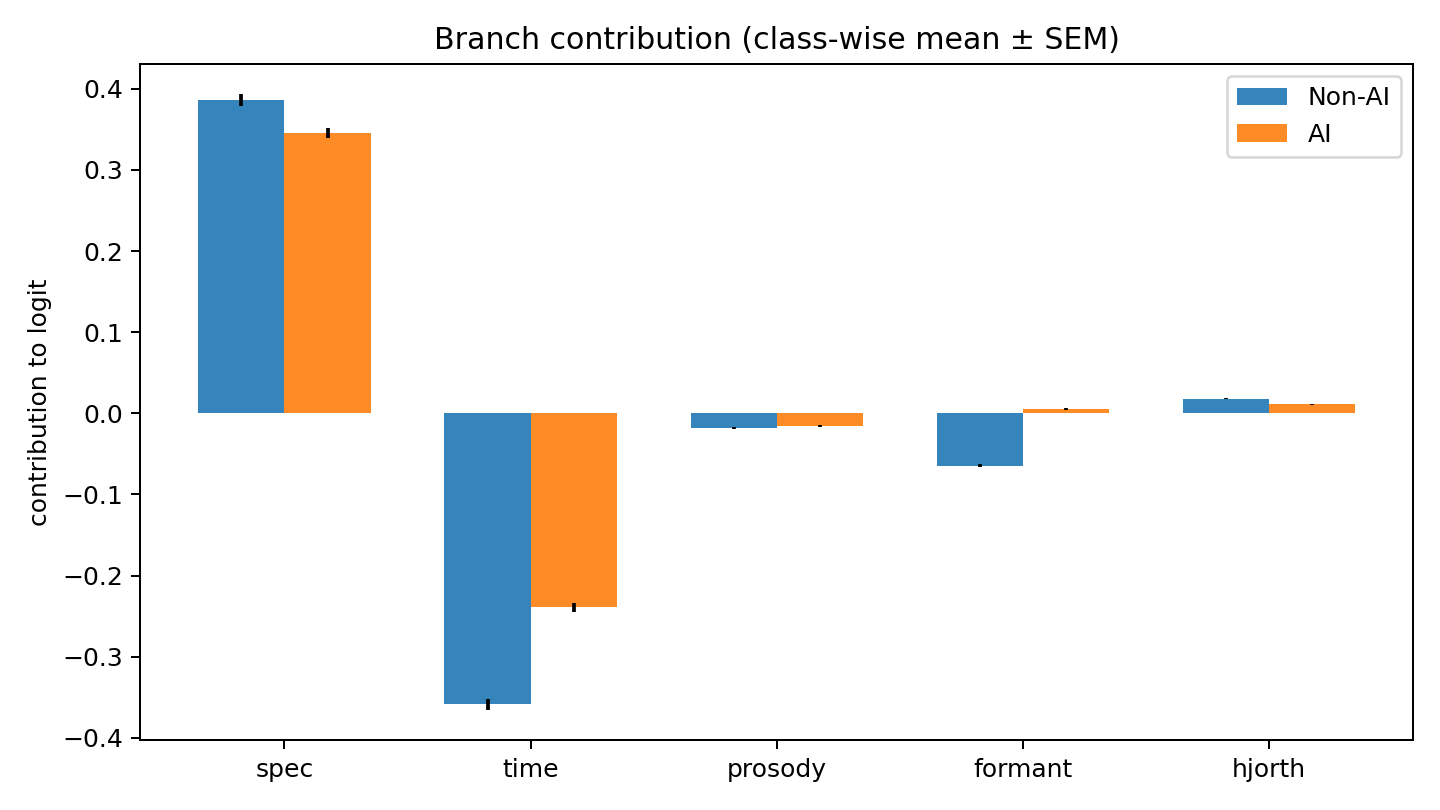
\includegraphics[width=.75\linewidth]{images_in_paper/contrib_means_by_class.png}
  \caption{不同分支在 AI 与非 AI 样本上的平均 logit 贡献（均值 $\pm$ SEM）。}
  \label{fig:contrib_means}
\end{figure}

为了考察分支贡献的相关性，我们计算了样本层面的皮尔逊相关系数矩阵（图~\ref{fig:contrib_corr}）。
结果显示，\texttt{spec} 与 \texttt{time} 分支呈显著负相关，
表明它们在多数样本的决策中存在一定的“对冲”关系——当一个分支强烈推动向 AI 方向时，另一个分支往往抑制该判别。
此外，\texttt{prosody} 与 \texttt{time}、\texttt{formant} 的正相关，说明这些分支在部分样本中可能协同作用。

\begin{figure}[H]
  \centering
  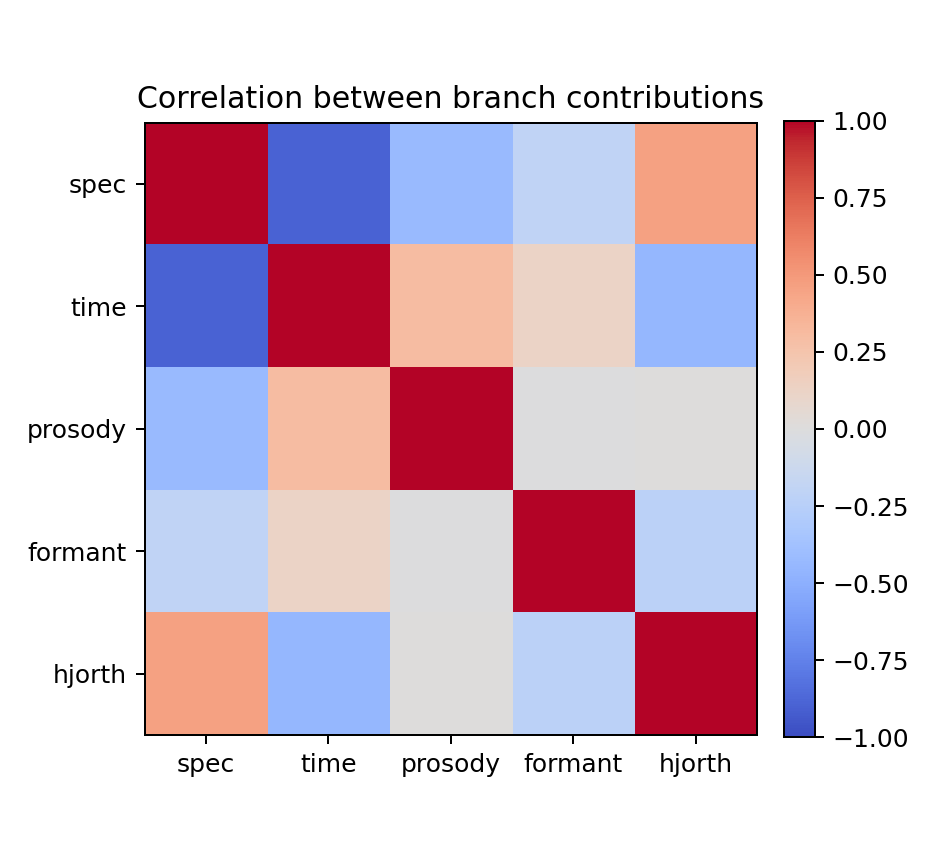
\includegraphics[width=.5\linewidth]{images_in_paper/contrib_correlation.png}
  \caption{各分支 logit 贡献的相关性矩阵（皮尔逊相关系数）。}
  \label{fig:contrib_corr}
\end{figure}

图~\ref{fig:contrib_violin} 给出了所有样本的分支贡献分布。
可以看出，\texttt{time} 分支的贡献分布跨度最大，从强负到强正均有覆盖，说明它在部分样本中具有极高的判别权重，而在另一些样本中几乎不参与判别；
\texttt{spec} 分支则分布相对集中且整体偏正，体现了其在多数样本中稳定推高 AI 判别的趋势；
\texttt{formant} 分支分布较分散，但极端值较多，可能在某些特定声学风格下起关键作用。

\begin{figure}[H]
  \centering
  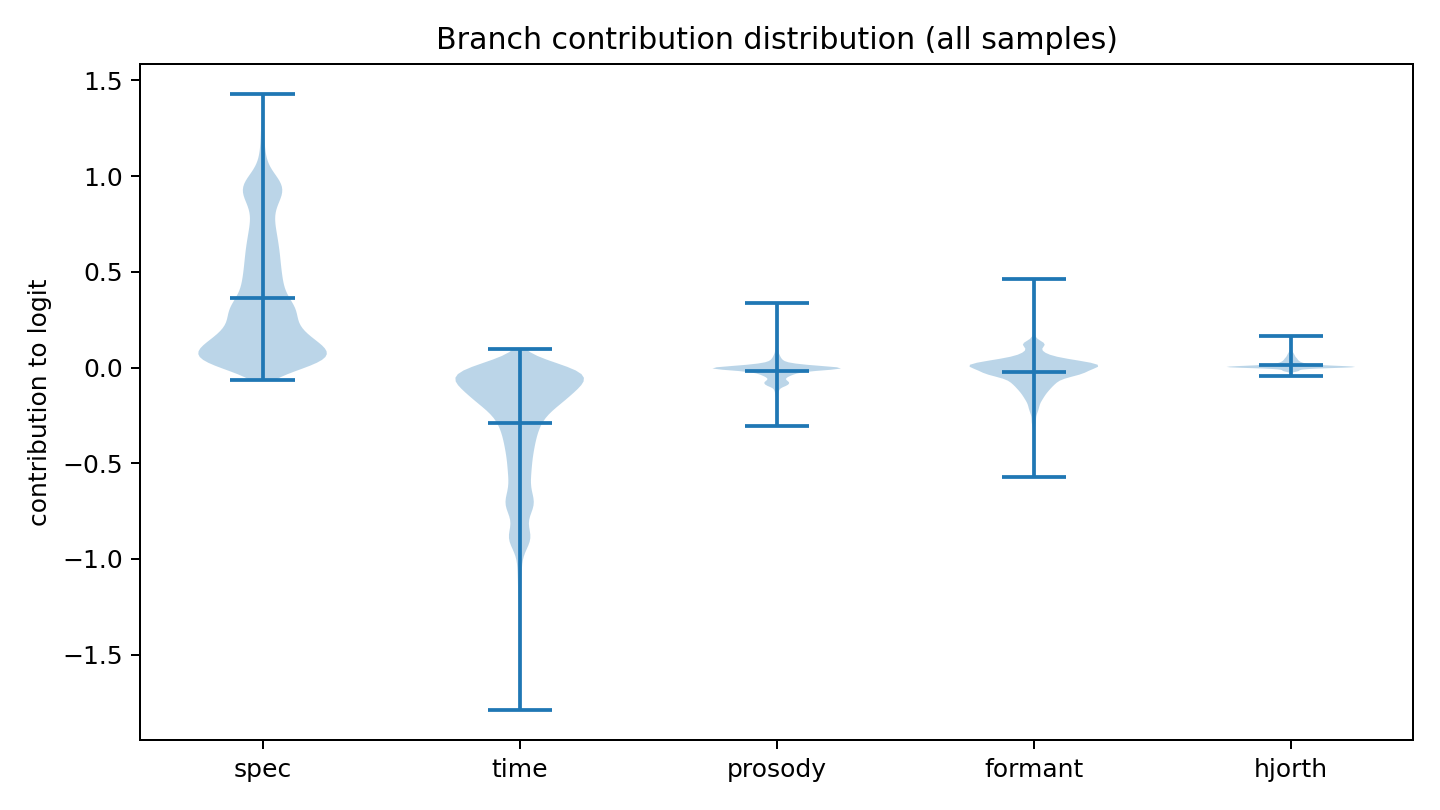
\includegraphics[width=.75\linewidth]{images_in_paper/contrib_violin_all.png}
  \caption{各分支 logit 贡献的分布（所有样本）。}
  \label{fig:contrib_violin}
\end{figure}

为了量化各分支的决策能力，本文通过 AUC、ACC 及 Fisher 比率（用于衡量类间分离度）
对各分支特征嵌入进行评估。
% 实验结果如表 \ref{tab:branch-eval} 所示。

定量分析表明，各分支的鲁棒性与其判别能力高度相关。
其中，时域分支（AUC: $0.825 \pm 0.008$, ACC: $0.763 \pm 0.003$, Fisher: $0.132$）
与共振峰分支（AUC: $0.816 \pm 0.008$, ACC: $0.741 \pm 0.010$, Fisher: $0.091$）展现出最强的判别力，
显著优于 Prosody（AUC: $0.719$, Fisher: $0.007$）及 Hjorth（AUC: $0.696$, Fisher: $0.005$）等分支。
这一结论解释了模型决策逻辑：融合推理主要依赖时域动态与人声共振峰布局。
当这两类关键特征遭受结构性扰动时，分类置信度会出现显著波动。

\begin{figure}[H]
  \centering
  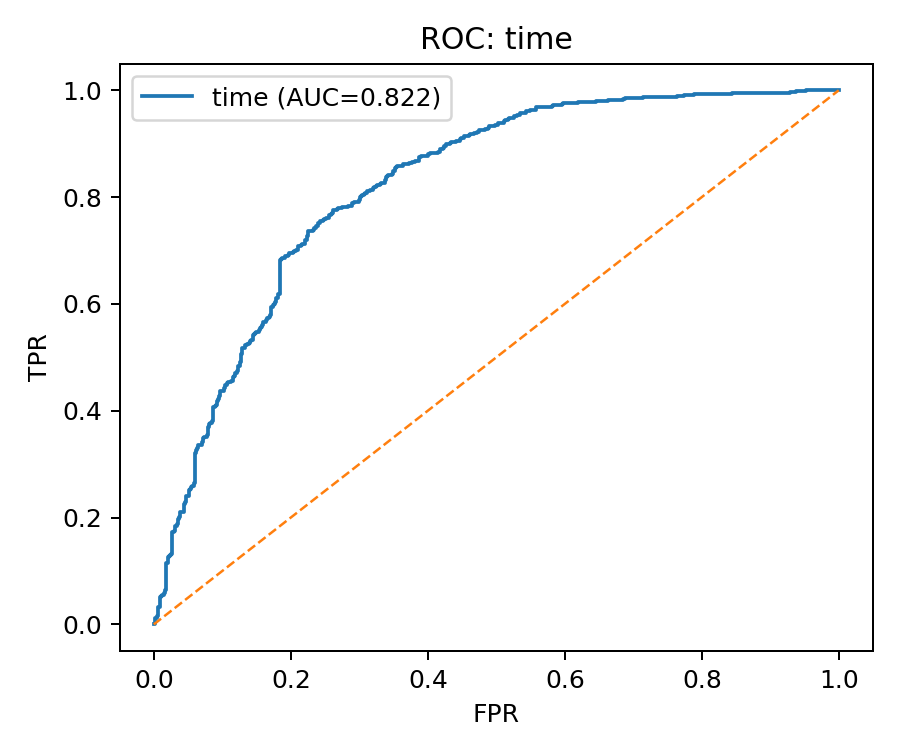
\includegraphics[width=.45\linewidth]{images_in_paper/roc_time.png}
  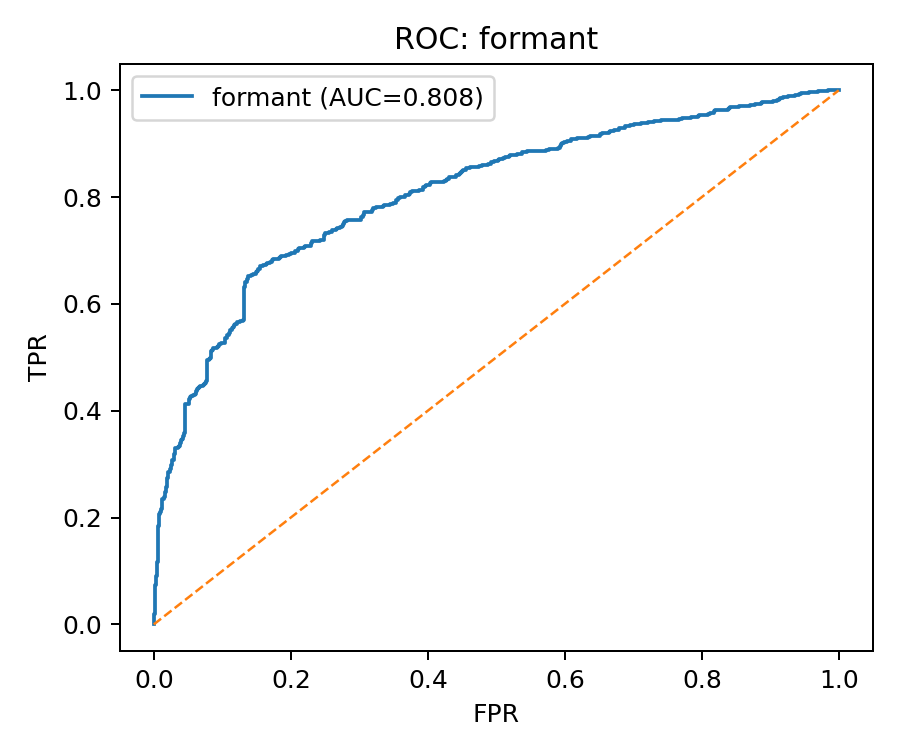
\includegraphics[width=.45\linewidth]{images_in_paper/roc_formant.png}
  \caption{时域分支与 formant 分支 ROC 曲线。}
  \label{fig:roc}
\end{figure}

\begin{figure}[H]
  \centering
  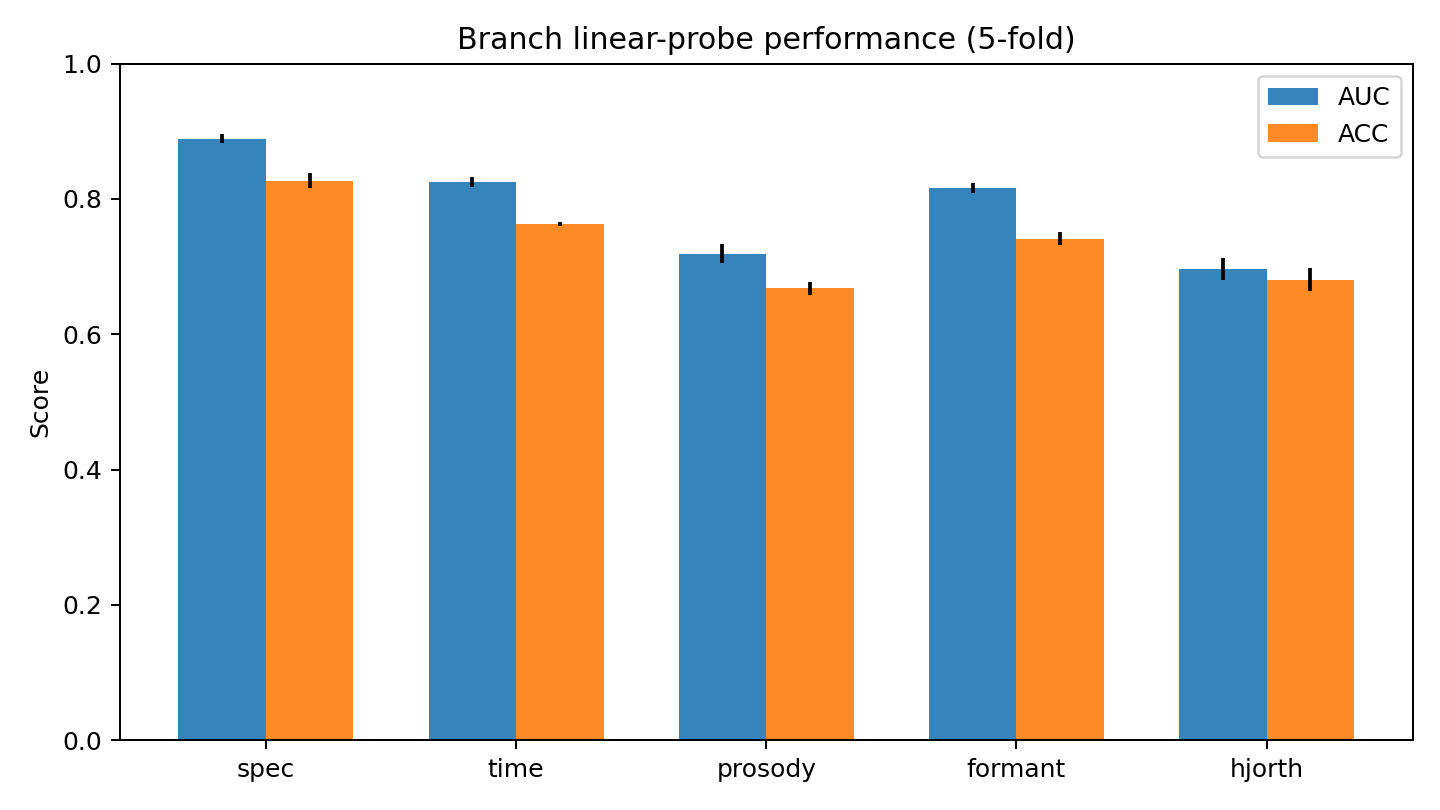
\includegraphics[width=.32\linewidth]{images_in_paper/branch_metrics_auc_acc.png}
  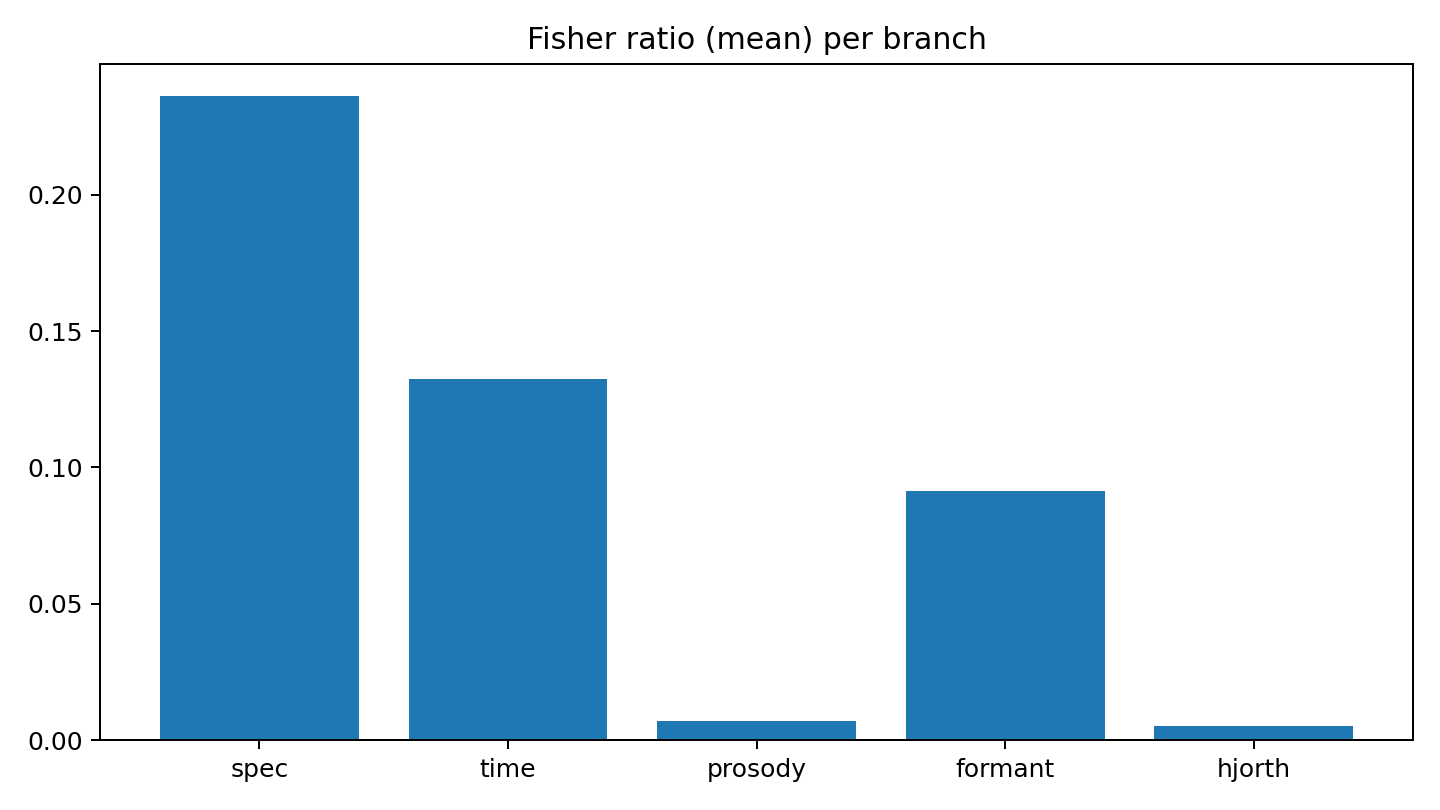
\includegraphics[width=.32\linewidth]{images_in_paper/branch_fisher.png}
  \caption{分支可分性定量指标：AUC/ACC（中）、Fisher 比率（右）。}
  \label{fig:branch_silhouette}
  \label{fig:branch_aucacc}
  \label{fig:branch_fisher}
\end{figure}

\end{document}
